\section{Resultados}
\label{sec:resultados}

\subsection{Variação do Intervalo de Heartbeat (\texorpdfstring{$N=3$}{N=3})}
A Tabela~\ref{tab:resultados_hbeat} apresenta os dados obtidos com o script
\texttt{run\_experiment.py} isolando o tempo de término do contêiner. O intervalo
de 1 s resultou em tempo médio de convergência de 1,186 s, consistente com a
bateria de escalabilidade para $N=3$ (1,177 s). Nos intervalos de 2 s e 3 s, a
convergência aumentou proporcionalmente para 2,932 s e 4,900 s, comprovando a
relação linear entre o período de verificação e a detecção de falhas ($2 \times T$).

\begin{table}[!t]
\centering
\setlength{\tabcolsep}{3.2pt}
\caption{Resultados do experimento com variação de heartbeat ($N=3$)}
\label{tab:resultados_hbeat}
\begin{tabular}{c c c c c c c c}
\toprule
Heartbeat & Rep. & Normal & Falha & Média & DP & p50 & p95 \\
(s) & & & & (s) & (s) & (s) & (s) \\
\midrule
1 & 3 & 1,0 & 1,0 & 1,186 & 0,436 & 0,973 & 1,616 \\
2 & 3 & 1,0 & 1,0 & 2,932 & 0,118 & 2,869 & 3,048 \\
3 & 3 & 1,0 & 1,0 & 4,900 & 0,064 & 4,935 & 4,938 \\
\bottomrule
\end{tabular}
\end{table}

\subsection{Escalabilidade e Contagem de Mensagens (\texorpdfstring{$N \in \{3, 5, 7, 10\}$}{N in {3, 5, 7, 10}})}
A Tabela~\ref{tab:resultados_bateria} sintetiza o comportamento do cluster no
cenário de escalabilidade com $T=1{,}0$ s e limiar de 2 falhas (10 repetições
independentes por configuração), cronometrando a latência imediatamente após a
interrupção do contêiner.

\begin{table}[!t]
\centering
\caption{Escalabilidade e mensagens ($T=1{,}0$ s)}
\label{tab:resultados_bateria}
\begin{tabular}{c c c c c c}
\toprule
$N$ Nós & Rep. & Média (s) & DP (s) & p95 (s) & Total Msgs \\
\midrule
3  & 10 & 1,177 & 0,123 & 1,325 & 5,7  \\
5  & 10 & 1,013 & 0,349 & 1,347 & 12,0 \\
7  & 10 & 1,221 & 0,155 & 1,449 & 25,1 \\
10 & 10 & 1,149 & 0,127 & 1,336 & 78,8 \\
\bottomrule
\end{tabular}
\end{table}

Ao isolar o tempo de parada do contêiner, observa-se que a latência média de
convergência algorítmica permaneceu praticamente constante entre 1,01 s e 1,22 s
para todos os tamanhos de cluster. Isso comprova que, em rede local, o tempo de
transmissão gRPC é desprezível frente ao período de amostragem dos heartbeats.

A Figura~\ref{fig:messages} ilustra a quantidade média de mensagens trocadas,
evidenciando a curvatura quadrática esperada do algoritmo Bully. No cenário de
escalabilidade pura, o volume médio cresceu de 5,7 mensagens para $N=3$ até 78,8
mensagens para $N=10$. No cenário completo com recuperação (\textit{baseline}), a troca
total média foi de 8,0 mensagens para $N=3$; 25,8 para $N=5$; 33,0 para $N=7$;
e 69,8 para $N=10$.
A Figura~\ref{fig:convergence} apresenta a comparação da latência média de
convergência em todos os cenários.

\begin{figure}[!t]
\centering
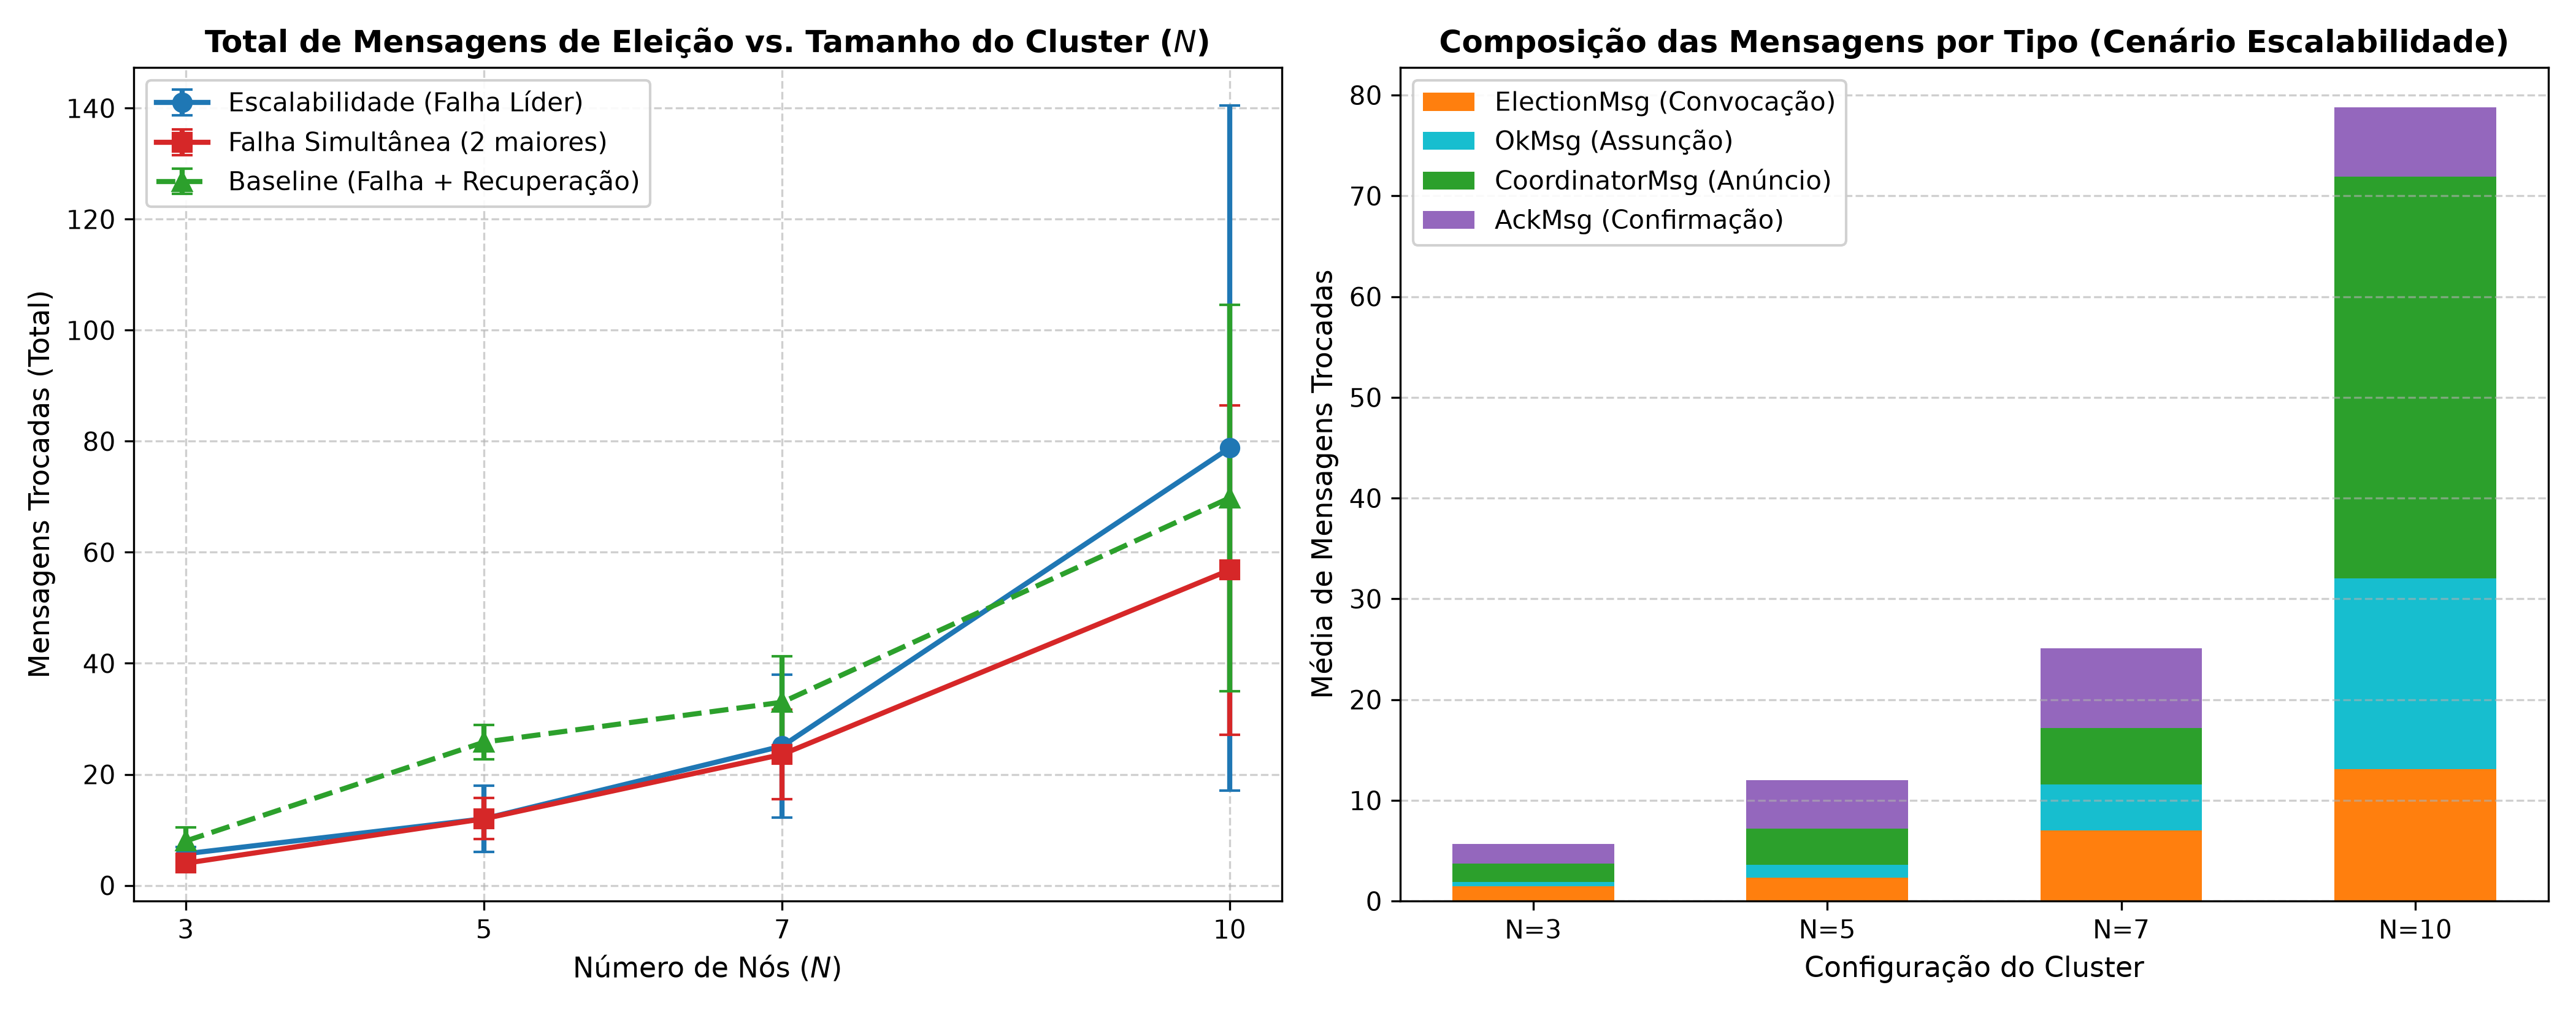
\includegraphics[width=\columnwidth]{images/battery_message_scaling.png}
\caption{Crescimento do volume de mensagens trocadas no algoritmo Bully em função do tamanho do cluster ($N \in \{3, 5, 7, 10\}$).}
\label{fig:messages}
\end{figure}

\begin{figure}[!t]
\centering
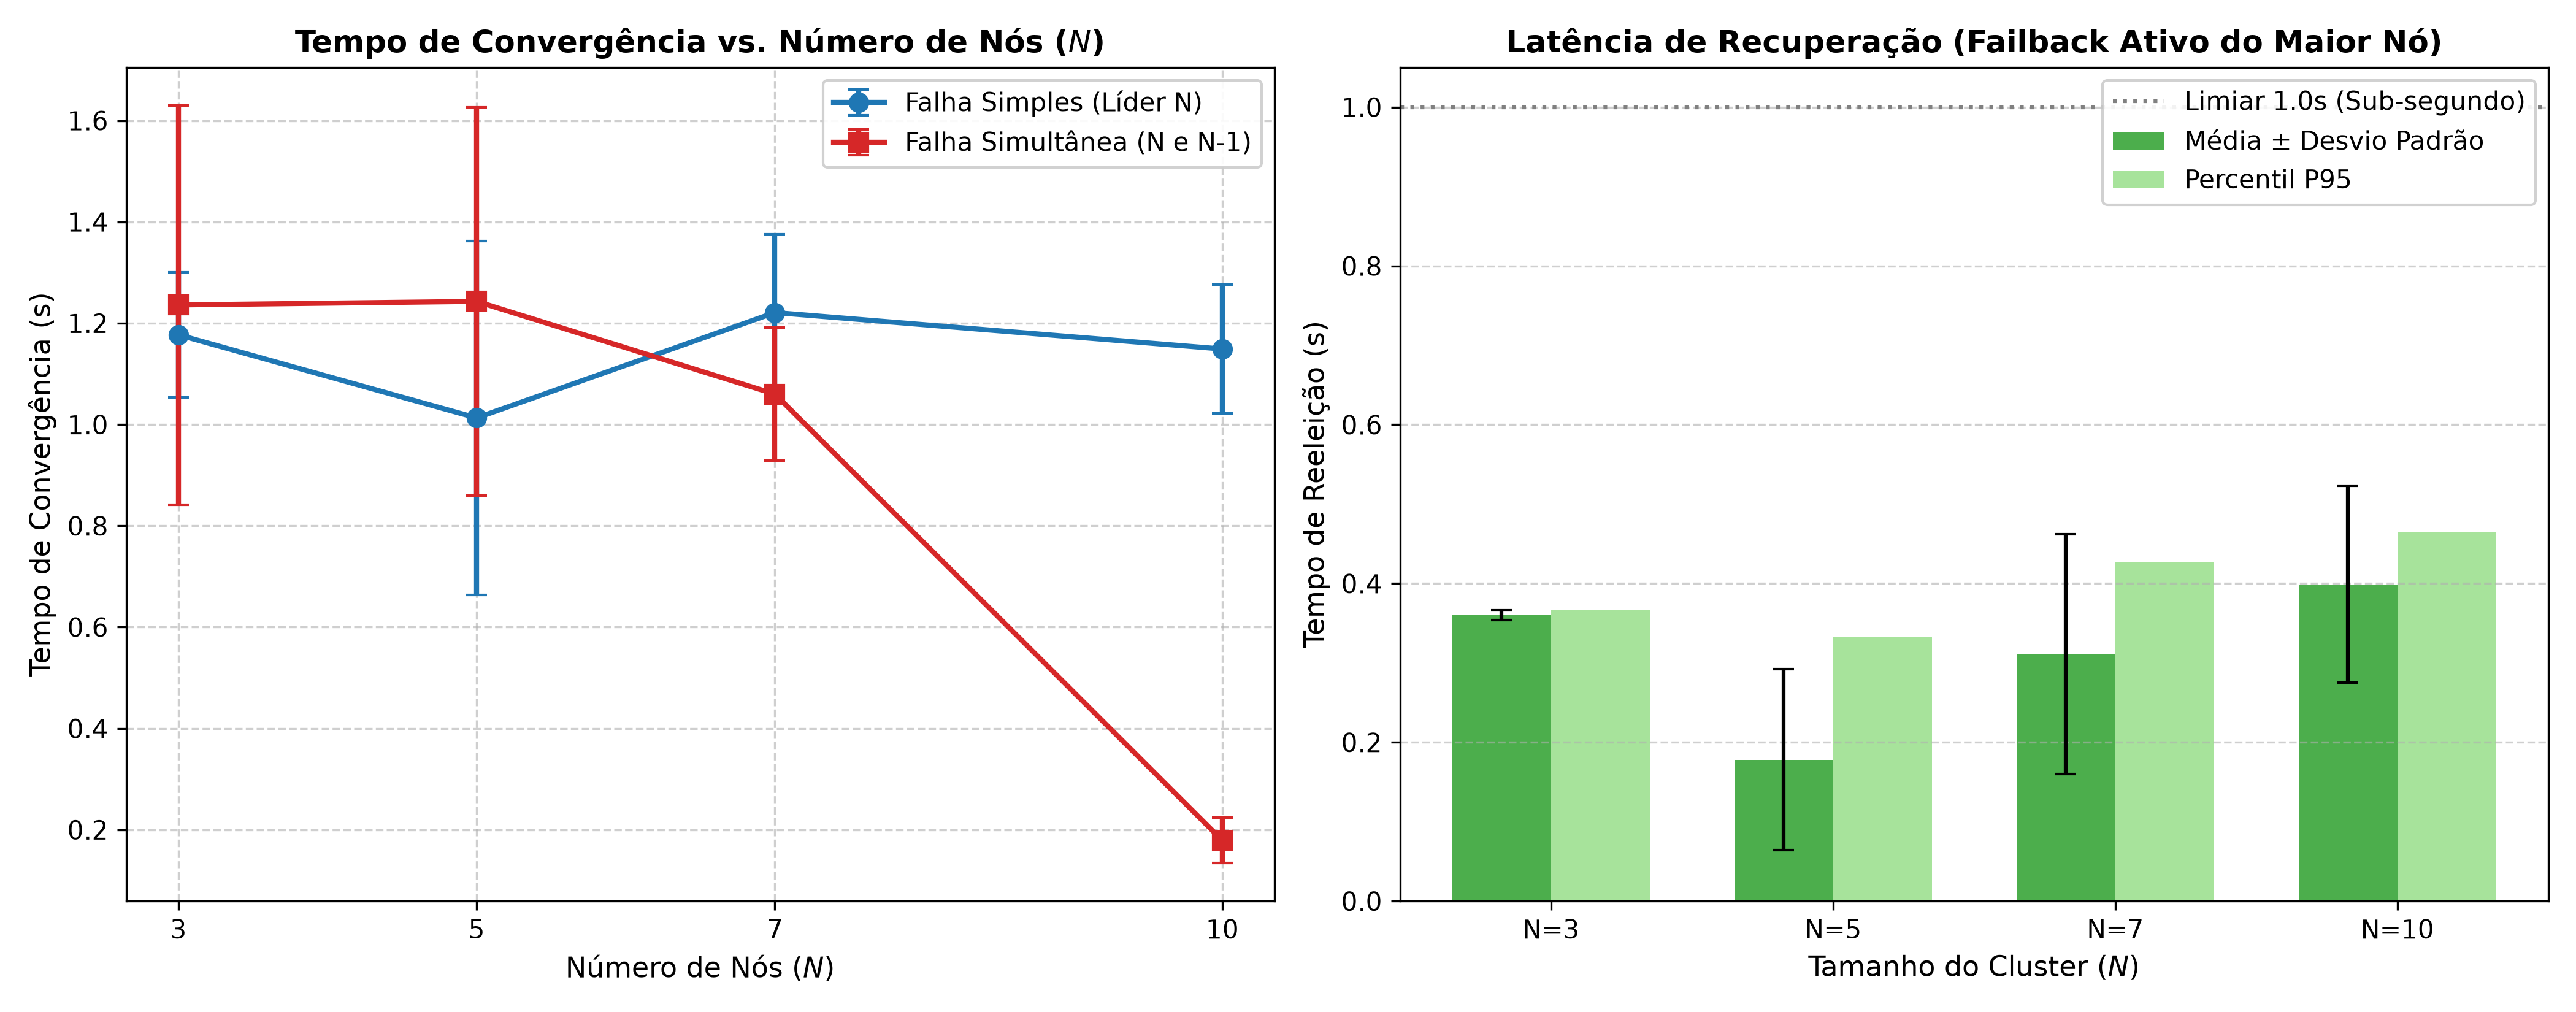
\includegraphics[width=\columnwidth]{images/battery_convergence_scaling.png}
\caption{Latência média de convergência para diferentes cenários e tamanhos de cluster.}
\label{fig:convergence}
\end{figure}

\subsection{Cenários de Falhas Complexas}
No cenário de falhas simultâneas, os contêineres $N$ e $N-1$ foram parados
concomitantemente. Em 100\% das execuções, o nó $N-2$ assumiu com sucesso a
liderança, sem ocorrência de impasses ou bloqueios.

No cenário de falha intermediária ($\lfloor N/2 \rfloor$), nenhuma nova eleição
foi disparada e o coordenador principal permaneceu inalterado e respondendo em
todas as repetições, confirmando a robustez do detector diante de falhas de nós
não coordenadores.
